\chapter{Desenvolvimento do projeto}
\label{chap:metod}
Este capítulo detalha o processo inicial de desenvolvimento do site de portfólio fotográfico, desde a concepção da ideia até a definição do design. Serão apresentados a ideação do projeto, as especificações técnicas e as funcionalidades implementadas.
\subsection{Metodologia do projeto}
A metodologia utilizada para o desenvolvimento deste projeto foi baseada no modelo \textit{Waterfall} (cascata), que é um modelo de desenvolvimento de software linear e sequencial. Este modelo é caracterizado por fases distintas, onde cada fase deve ser concluída antes do início da próxima. As fases do modelo \textit{Waterfall} incluem: requisitos, design, implementação, verificação e manutenção.

\section{Ideação}
Nesta seção será apresentada a fase de concepção inicial do projeto, incluindo o levantamento de necessidades do cliente, as referências visuais discutidas, os objetivos definidos para o site e as primeiras decisões relacionadas à estrutura e funcionalidades da plataforma. Serão abordados os encontros realizados com o cliente, os principais insumos obtidos a partir do workshop e como essas informações foram transformadas em requisitos e diretrizes para o design e desenvolvimento do site institucional.

%escrever oq sera apresentado

\subsection{Arquitetura Geral}
A arquitetura geral, apresentada na Figura \ref{fig:Arquitetura geral}, relaciona de modo geral a interface do usuário com a estrutura de apresentação do conteúdo e com os serviços externos integrados ao site. Neste contexto, a interface do usuário representa o ponto de acesso direto ao sistema por meio de navegadores em dispositivos móveis e desktops, permitindo a navegação entre páginas, visualização do portfólio e envio de mensagens de contato. A camada de serviços externos inclui integrações como formulários por e-mail (via Formspree) e redes sociais, como o Instagram.

 \begin{figure} [h!]	
    \centering

    \caption{Arquitetura Geral}
    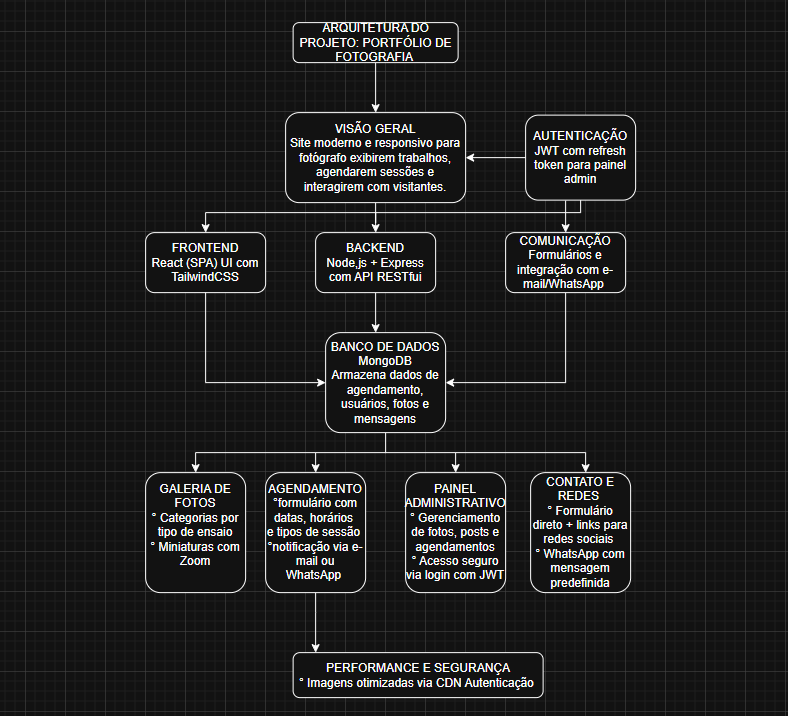
\includegraphics[width=0.8\textwidth]{Figures/Arquitetura_do_projeto.png}
    \caption*{Fonte: Autoria própria.}
    \label{fig:Arquitetura geral}
\end{figure}	

Para a estrutura de gerenciamento do site, utilizou-se um conjunto de tecnologias web padrão, incluindo HTML5, CSS3 e JavaScript no front-end. Essa camada é responsável por controlar as principais funcionalidades do sistema: exibição da galeria de fotos com filtros por categoria, navegação entre seções, exibição de informações institucionais, envio de mensagens por meio do formulário de contato e o sistema de agendamento de ensaios fotográficos. Este último permite que o usuário selecione uma data, horário e tipo de ensaio, com envio de confirmação por e-mail.

\subsection{Requisitos técnicos}
Os requisitos técnicos do site foram definidos com base nas demandas do cliente identificadas durante o workshop de levantamento de requisitos. A equipe utilizou uma abordagem inspirada no \textit{Quality Function Deployment} (QFD) para converter as necessidades funcionais e expectativas em características técnicas específicas que pudessem ser implementadas de forma objetiva e eficiente. Os principais requisitos definidos para o sistema foram:

\begin{itemize}
    \item O site deve ser 100\% responsivo, garantindo uma boa experiência em smartphones, tablets e desktops;
    \item As imagens devem ser otimizadas para carregamento rápido, com uso de técnicas como compressão e \textit{lazy loading};
    \item O layout deve seguir uma identidade visual alinhada à preferência do cliente (preto, branco e dourado), com foco em simplicidade e elegância;
    \item A galeria deve permitir filtragem por categorias (casamento, ensaio, corporativo, etc.);
    \item Deve ser possível realizar o agendamento de ensaios fotográficos com data, horário e tipo de serviço;
    \item O formulário de contato deve ser integrado ao e-mail do cliente e conter botão de WhatsApp;
    \item O sistema deve enviar confirmações de agendamento automaticamente por e-mail;
    \item O tempo médio de carregamento das páginas não deve ultrapassar 3 segundos;
    \item O código-fonte deve ser organizado, documentado e versionado com GitHub;
    \item O site deve permitir manutenção e expansão futura, como adição de blog ou painel administrativo.
\end{itemize}
%desdobramento da função qualidade
% \subsection{Quality Function Deployment}
% \textit{Quality Function Deployment} é uma ferramenta de qualidade que auxilia na conversão das demandas do cliente em características de qualidade do produto. Dessa forma, no primeiro ciclo do QFD foram analisados os requisistos do cliente e os requisitos técnicos necessários, sinalizando os pontos mais importantes e as relações entre estes. O resultado foi exposto na \ref{fig:QFD}

% \begin{figure} [h!]	
%     \centering
%     \caption{ Primeiro ciclo QFD}
%     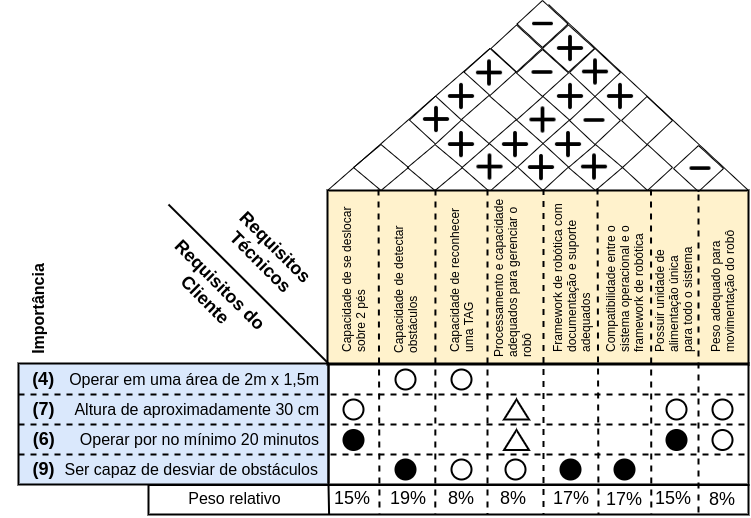
\includegraphics[width=0.8\textwidth]{Figures/QFD}
%     \caption*{Fonte: Autoria própria.}
%     \label{fig:QFD}
% \end{figure}
%  Através do QFD foi possível observar 

% % %--------- NEW SECTION ----------------------
% % \section{Interface do Usuário}
% % \label{sec:ui}
% % \lipsum[1]

% % %--------- NEW SECTION ----------------------
% % \section{Simulação do sistema}
% % \label{sec:sim}
% % \lipsum[2-4]
\subsection{Modelagem dos processos}

\begin{figure} [h!]	
    \centering

    \caption{Modelo esquemático dos processos}
    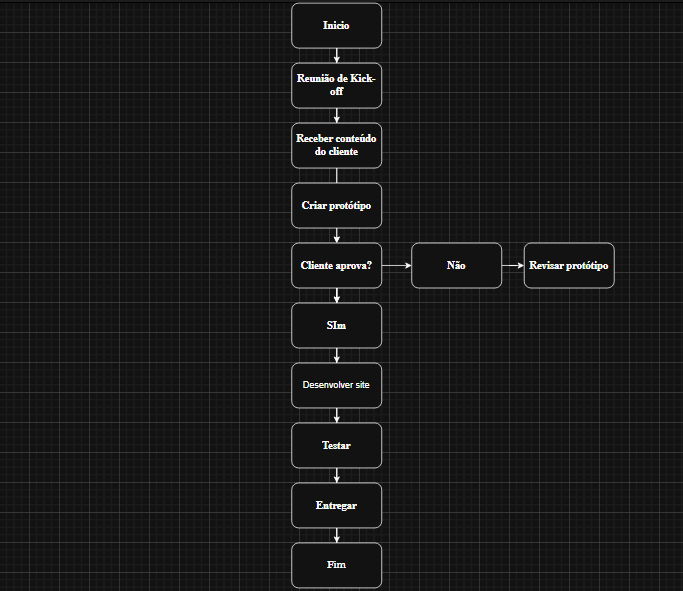
\includegraphics[width=0.8\textwidth]{Figures/modelo_esquematico_dos_processos.png}
    \caption*{Fonte: Autoria própria.}
    \label{fig:modelagem_dos_processos}
\end{figure}